\documentclass{beamer}
\usepackage{HECbeamer}
\usepackage{icomma}
\newcommand{\AIC}{\textsf{AIC}}
\newcommand{\BIC}{\textsf{BIC}}
% \usepackage{pgfpages}
% \pgfpagesuselayout{4 on 1}[letterpaper, landscape, border shrink=5mm]
\title[\color{white}{MATH 60604 \S~4g - Termes de décalage}]{\texorpdfstring{MATH 60604 \\Modélisation statistique \\ \S~4g - Taux et termes de décalage}{MATH 60604 \\Modélisation statistique \\ \S~4g - Taux et termes de décalage}}
\author{Léo Belzile}
\institute{HEC Montréal\\
Département de sciences de la décision}
\date{} 

\begin{document}
\frame{\titlepage}
\begin{frame}[fragile]
\frametitle{Décalage et comparaisons de dénombrement}
\bi
\item Jusqu'à présent, nous avons supposé que la variable de dénombrement $Y$  était \alert{comparable} d'un individu à l'autre.
\bi 
\item Dans l'exemple d'achats, $Y_i$ représentait le nombre de fois que le sujet $i$ avait acheté le produit dans le mois suivant l'étude.
\ei
\item  Et si la période de suivi variait d'un individu l'autre?
\bi
\item le nombre d'accidents de travail dans une entreprise pour une période donnée dépend du nombre d'employés.
\item le nombre de cancer par région dépend du nombre d'habitants.
\ei
\ei
Si les nombres ne sont pas comparables, on peut considérer les \textbf{taux} (nombre d'achats par mois, nombre d'accident par employé, etc.)


Si on modélise le taux avec le modèle de Poisson, ce dernier est adéquat \textbf{seulement} si le taux est \alert{faible}.

\end{frame}
% 
% \begin{frame}[fragile]
% \frametitle{Making the counts comparable}
% \bi
% \item In all these examples, the variable $Y$ is not comparable between subject (between lines of the data file)
% \item Talking about the ``number of\ldots'' doesn't mean anything if we don't know the follow-up time of the subject, the number of employees in a business, the size of the cookie, etc.
% \item Instead, we can talk about a \alert{rate}:
% \bi
% 
% \item The rate of purchase (number of purchases per month)
% \item The work accident rate (number of accidents per employee)
% \item The chocolate chip rate (number of chocolate chips per square centimetre of a cookie)
% \ei
% \ei
% \end{frame}

\begin{frame}[fragile]
\frametitle{Données sur les accidents de la route}
La \textit{National Highway Traffic Safety Administration} (NHTSA) compile des statistiques sur le nombre de morts sur les routes aux États-Unis. Les données \texttt{accident} dénombre les décès en $2010$ et en $2018$ par États, recensés par régions géographiques (\texttt{region}) telles que définies par la NHTSA et catégorisées selon le \texttt{moment} où l'accident a eu lieu (jour ou nuit).

\bi
\item Soit $Y_i$ le nombre de décès à un moment donné durant une année donnée pour la région $i$;
\item Soit $N_i$ le nombre d'habitants dans la région $i$.
\ei
Notre objectif est d'estimer la relation entre nombre d'accident fatal selon le moment de la journée et l'année.
\end{frame}
\begin{frame}
 \begin{center}
  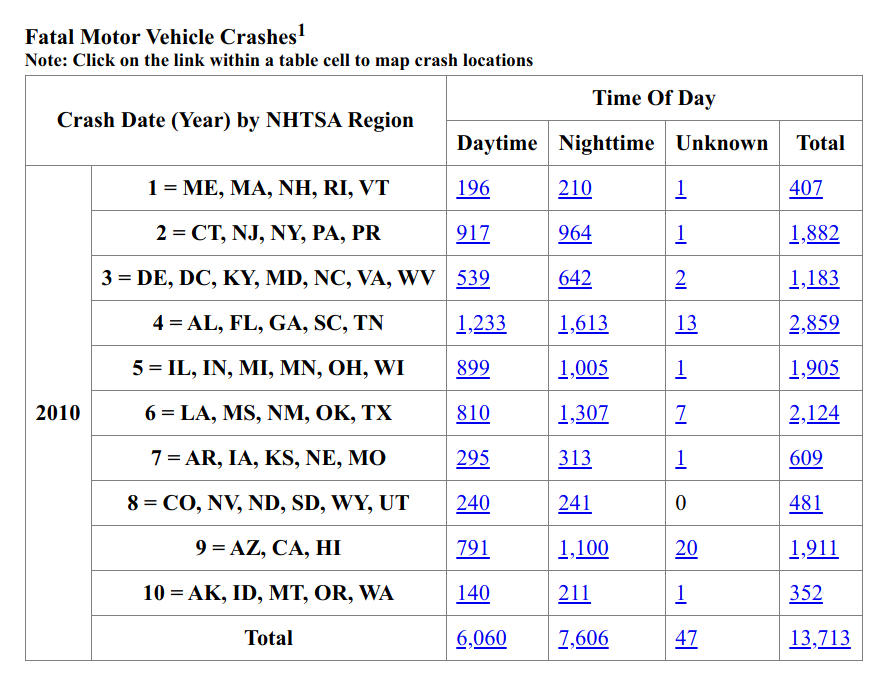
\includegraphics[width = 0.8\linewidth]{img/c4/crash.png}
 \end{center}
\end{frame}
\begin{frame}[fragile]
\frametitle{Accidents de la route et décalage}
\bi
\item Si on ignore la taille de la population, le modèle de régression de Poisson (ou binomiale négative) s'écrirait
\begin{align*}
\ln(\mu_i)=\ln\{\E{Y_i}\}=\beta_0 + \beta_1 \code{moment} + \beta_2 \code{annee}
\end{align*}
\item Si on prend en compte la taille de la population, cela revient à modéliser le taux $Y_i/N_i$ plutôt que $Y_i$.
\item On fixe
\begin{align*}
\ln\left\{\frac{\E{Y_i}}{N_i}\right\}&=\beta_0 +\beta_1 \code{moment} + \beta_2 \code{annee}
\intertext{ou de manière équivalente}
\ln\left\{\E{Y_i}\right\}&=\beta_0 + \beta_1 \code{moment} + \beta_2 \code{annee}+\ln( N_i)
\end{align*}
\item Le terme $\ln(N_i)$ est un \alert{\textbf{terme de décalage}}; une variable explicative incluse sans paramètre.
\ei
\end{frame}

\begin{frame}[fragile]
\frametitle{Régression binomiale négative pour \texttt{accidents}}

\begin{tcolorbox}[colback=white, colframe=hecblue, title=Code \SASlang{} pour inclure un terme de décalage]
{\small
\begin{verbatim}
data accident;
set modstat.accident;
logpopn=log(popn);
run;
proc genmod data=accident;
class moment(ref="jour") annee(ref="2010");
model nmorts=moment annee / dist=negbin link=log 
    offset=logpopn type3 lrci;
run;
\end{verbatim}
}
\end{tcolorbox}
{\footnotesize 

L'option \texttt{offset} pourrait aussi être utilisée dans une régression de Poisson.



}
\begin{center}
 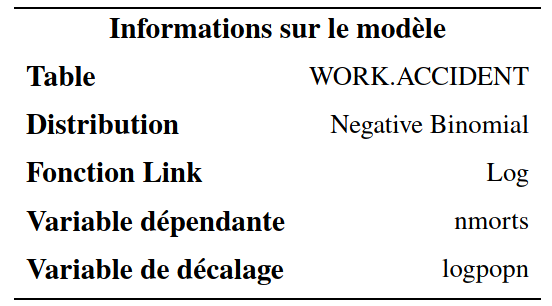
\includegraphics[width = 0.4\linewidth]{img/c4/diapos8-e9}
\end{center}

\end{frame}
\begin{frame}{Interprétation  des paramètres avec décalage}
\begin{center}
 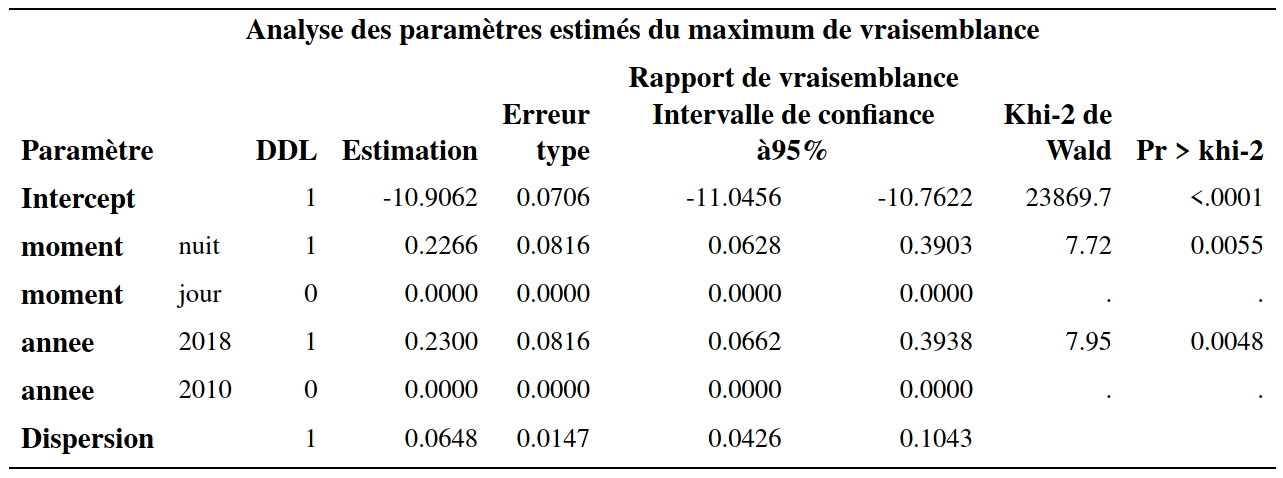
\includegraphics[width = 0.99\linewidth]{img/c4/diapos8-e10}
\end{center}
{\small 
\bi \item La variable de décalage $\ln(N)$ n'apparaît pas dans le tableau.
\item La statistique de déviance (sortie omise) est $40,269$ pour $37$ degrés de liberté (rapport de $1,09$). La valeur-$p$ correspondante est $0,327$, donc il n'y a pas de preuve que notre modèle est inadéquat.
\item Le taux de mortalité durant le jour en $2010$ est $\exp(\hat{\beta}_0)=\exp(-10,91)$ ou $1,83/100000$, soit un taux de $1,83$ décès par $100\,000$ habitants (avec intervalle de confiance à $95$\%  [$1,60, 2,12]\times 10^{-5}$).
\item On estime que la mortalité moyenne entre $2010$ et $2018$ augmente de $26$\%, puisque $\exp(0,23)=1,26$.
\ei
}
\end{frame}
\end{document}
